% !TEX TS-program = pdflatex
% !TEX encoding = UTF-8 Unicode
\documentclass[border=0mm]{standalone}
% packages
\usepackage{tikz}
\usetikzlibrary{patterns}
\usepackage{amsmath,amssymb}
\usepackage{bm}
\usepackage{pgfplots}
\pgfplotsset{compat=1.15}
% start document
\begin{document}
% generated by ROOT (CERN)
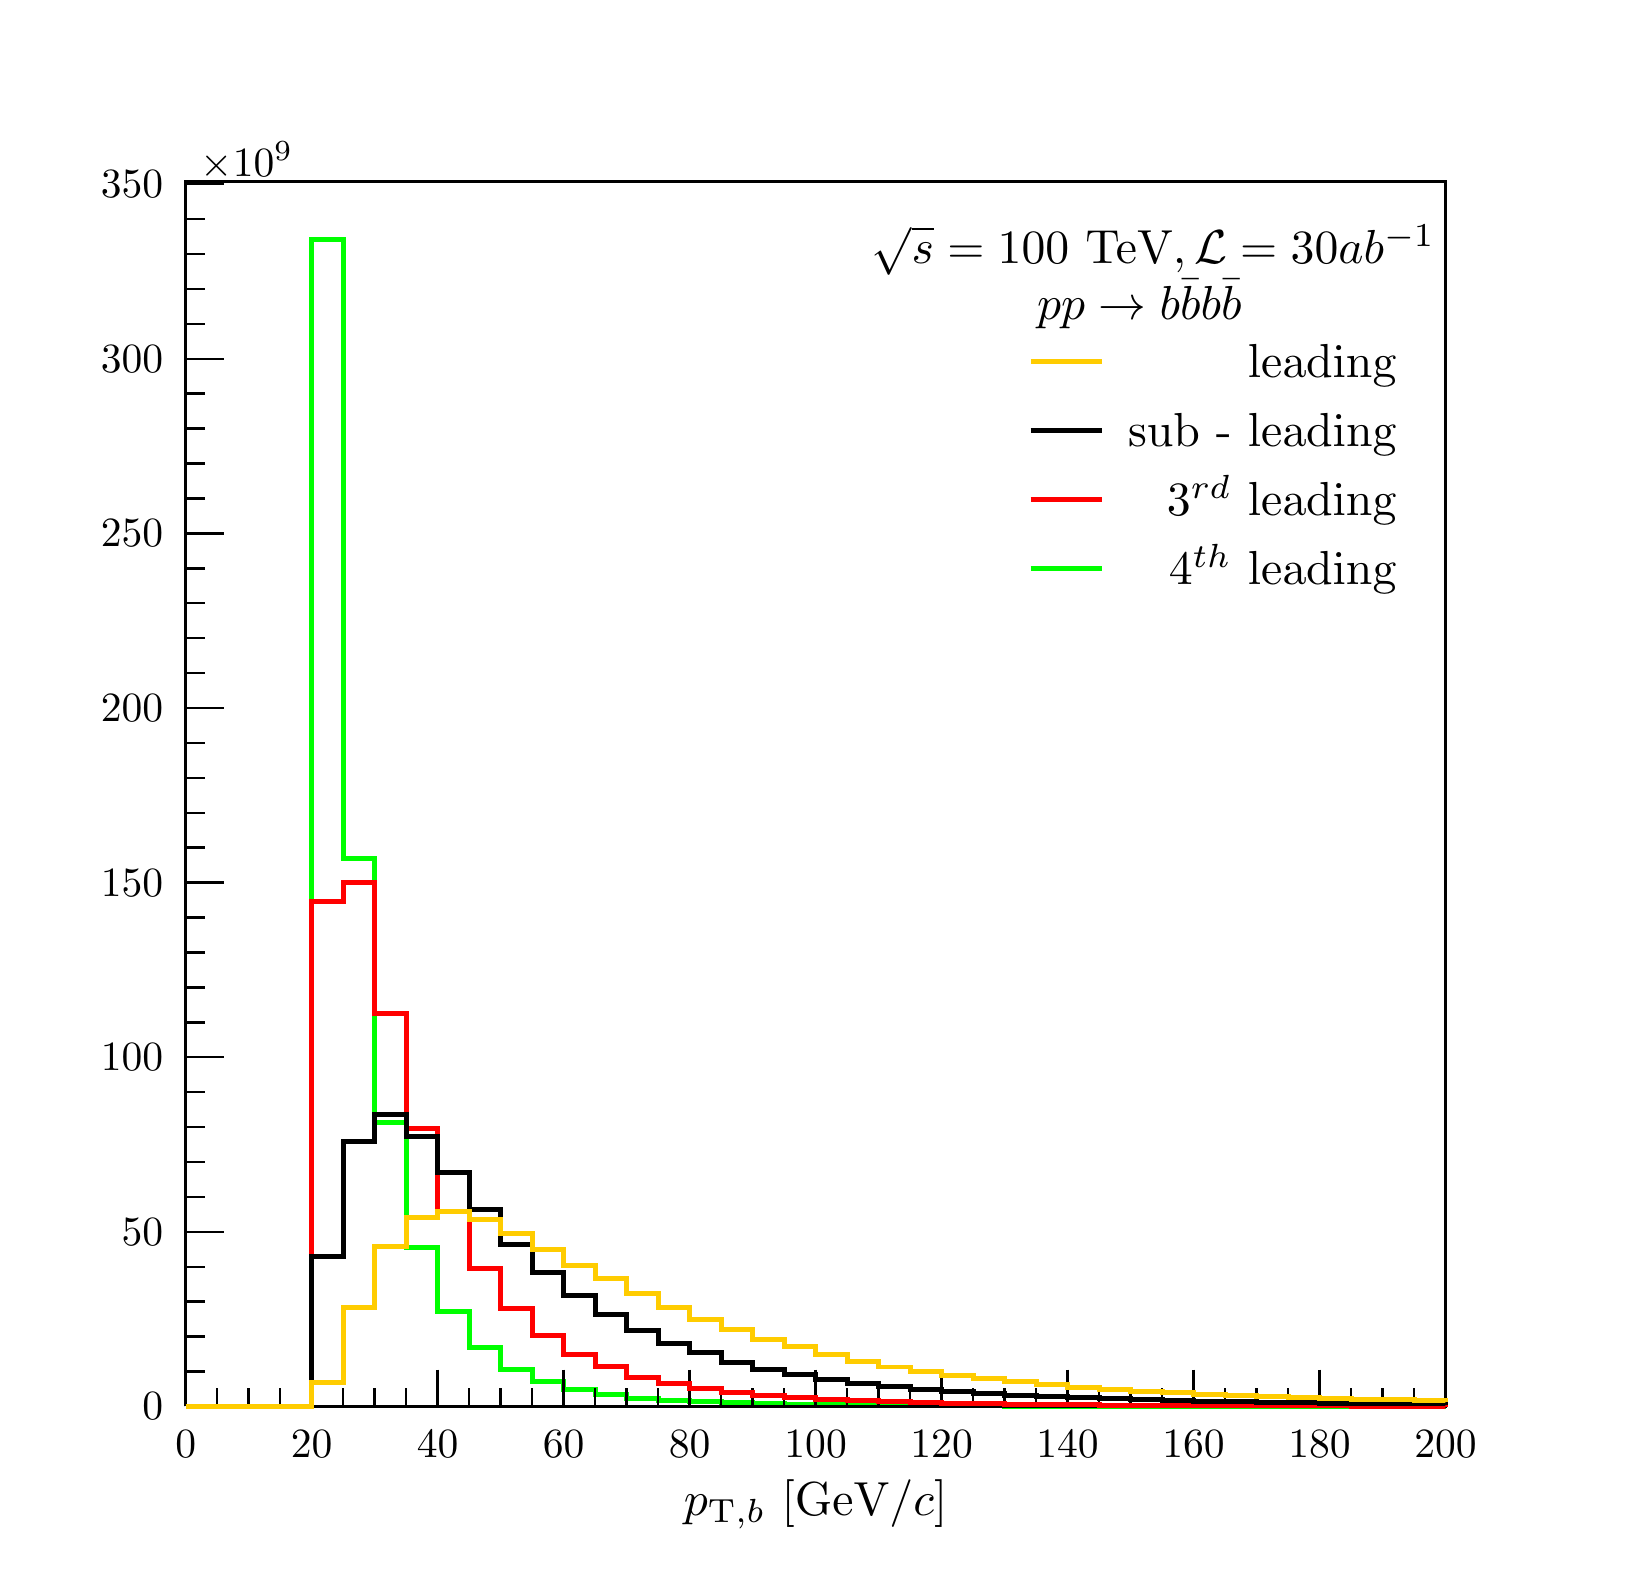
\begin{tikzpicture}
\pgfdeclareplotmark{cross} {
\pgfpathmoveto{\pgfpoint{-0.3\pgfplotmarksize}{\pgfplotmarksize}}
\pgfpathlineto{\pgfpoint{+0.3\pgfplotmarksize}{\pgfplotmarksize}}
\pgfpathlineto{\pgfpoint{+0.3\pgfplotmarksize}{0.3\pgfplotmarksize}}
\pgfpathlineto{\pgfpoint{+1\pgfplotmarksize}{0.3\pgfplotmarksize}}
\pgfpathlineto{\pgfpoint{+1\pgfplotmarksize}{-0.3\pgfplotmarksize}}
\pgfpathlineto{\pgfpoint{+0.3\pgfplotmarksize}{-0.3\pgfplotmarksize}}
\pgfpathlineto{\pgfpoint{+0.3\pgfplotmarksize}{-1.\pgfplotmarksize}}
\pgfpathlineto{\pgfpoint{-0.3\pgfplotmarksize}{-1.\pgfplotmarksize}}
\pgfpathlineto{\pgfpoint{-0.3\pgfplotmarksize}{-0.3\pgfplotmarksize}}
\pgfpathlineto{\pgfpoint{-1.\pgfplotmarksize}{-0.3\pgfplotmarksize}}
\pgfpathlineto{\pgfpoint{-1.\pgfplotmarksize}{0.3\pgfplotmarksize}}
\pgfpathlineto{\pgfpoint{-0.3\pgfplotmarksize}{0.3\pgfplotmarksize}}
\pgfpathclose
\pgfusepathqstroke
}
\pgfdeclareplotmark{cross*} {
\pgfpathmoveto{\pgfpoint{-0.3\pgfplotmarksize}{\pgfplotmarksize}}
\pgfpathlineto{\pgfpoint{+0.3\pgfplotmarksize}{\pgfplotmarksize}}
\pgfpathlineto{\pgfpoint{+0.3\pgfplotmarksize}{0.3\pgfplotmarksize}}
\pgfpathlineto{\pgfpoint{+1\pgfplotmarksize}{0.3\pgfplotmarksize}}
\pgfpathlineto{\pgfpoint{+1\pgfplotmarksize}{-0.3\pgfplotmarksize}}
\pgfpathlineto{\pgfpoint{+0.3\pgfplotmarksize}{-0.3\pgfplotmarksize}}
\pgfpathlineto{\pgfpoint{+0.3\pgfplotmarksize}{-1.\pgfplotmarksize}}
\pgfpathlineto{\pgfpoint{-0.3\pgfplotmarksize}{-1.\pgfplotmarksize}}
\pgfpathlineto{\pgfpoint{-0.3\pgfplotmarksize}{-0.3\pgfplotmarksize}}
\pgfpathlineto{\pgfpoint{-1.\pgfplotmarksize}{-0.3\pgfplotmarksize}}
\pgfpathlineto{\pgfpoint{-1.\pgfplotmarksize}{0.3\pgfplotmarksize}}
\pgfpathlineto{\pgfpoint{-0.3\pgfplotmarksize}{0.3\pgfplotmarksize}}
\pgfpathclose
\pgfusepathqfillstroke
}
\pgfdeclareplotmark{newstar} {
\pgfpathmoveto{\pgfqpoint{0pt}{\pgfplotmarksize}}
\pgfpathlineto{\pgfqpointpolar{44}{0.5\pgfplotmarksize}}
\pgfpathlineto{\pgfqpointpolar{18}{\pgfplotmarksize}}
\pgfpathlineto{\pgfqpointpolar{-20}{0.5\pgfplotmarksize}}
\pgfpathlineto{\pgfqpointpolar{-54}{\pgfplotmarksize}}
\pgfpathlineto{\pgfqpointpolar{-90}{0.5\pgfplotmarksize}}
\pgfpathlineto{\pgfqpointpolar{234}{\pgfplotmarksize}}
\pgfpathlineto{\pgfqpointpolar{198}{0.5\pgfplotmarksize}}
\pgfpathlineto{\pgfqpointpolar{162}{\pgfplotmarksize}}
\pgfpathlineto{\pgfqpointpolar{134}{0.5\pgfplotmarksize}}
\pgfpathclose
\pgfusepathqstroke
}
\pgfdeclareplotmark{newstar*} {
\pgfpathmoveto{\pgfqpoint{0pt}{\pgfplotmarksize}}
\pgfpathlineto{\pgfqpointpolar{44}{0.5\pgfplotmarksize}}
\pgfpathlineto{\pgfqpointpolar{18}{\pgfplotmarksize}}
\pgfpathlineto{\pgfqpointpolar{-20}{0.5\pgfplotmarksize}}
\pgfpathlineto{\pgfqpointpolar{-54}{\pgfplotmarksize}}
\pgfpathlineto{\pgfqpointpolar{-90}{0.5\pgfplotmarksize}}
\pgfpathlineto{\pgfqpointpolar{234}{\pgfplotmarksize}}
\pgfpathlineto{\pgfqpointpolar{198}{0.5\pgfplotmarksize}}
\pgfpathlineto{\pgfqpointpolar{162}{\pgfplotmarksize}}
\pgfpathlineto{\pgfqpointpolar{134}{0.5\pgfplotmarksize}}
\pgfpathclose
\pgfusepathqfillstroke
}
\definecolor{c}{rgb}{1,1,1};
\draw [color=c, fill=c] (0,0) rectangle (20,19.4486);
\draw [color=c, fill=c] (0,0) rectangle (20,19.4486);
\draw [color=c, fill=c] (2,1.94486) rectangle (18,17.5038);
\definecolor{c}{rgb}{0,0,0};
\draw [c,line width=0.9] (2,1.94486) -- (2,17.5038) -- (18,17.5038) -- (18,1.94486) -- (2,1.94486);
\definecolor{c}{rgb}{1,1,1};
\draw [color=c, fill=c] (2,1.94486) rectangle (18,17.5038);
\definecolor{c}{rgb}{0,0,0};
\draw [c,line width=0.9] (2,1.94486) -- (2,17.5038) -- (18,17.5038) -- (18,1.94486) -- (2,1.94486);
\definecolor{c}{rgb}{0,1,0};
\draw [c,line width=1.8] (2,1.94486) -- (2.4,1.94486) -- (2.4,1.94486) -- (2.8,1.94486) -- (2.8,1.94486) -- (3.2,1.94486) -- (3.2,1.94486) -- (3.6,1.94486) -- (3.6,16.7629) -- (4,16.7629) -- (4,8.9037) -- (4.4,8.9037) -- (4.4,5.55399) --
 (4.8,5.55399) -- (4.8,3.96418) -- (5.2,3.96418) -- (5.2,3.15006) -- (5.6,3.15006) -- (5.6,2.68927) -- (6,2.68927) -- (6,2.41541) -- (6.4,2.41541) -- (6.4,2.26519) -- (6.8,2.26519) -- (6.8,2.16314) -- (7.2,2.16314) -- (7.2,2.09583) -- (7.6,2.09583)
 -- (7.6,2.05134) -- (8,2.05134) -- (8,2.0255) -- (8.4,2.0255) -- (8.4,2.00496) -- (8.8,2.00496) -- (8.8,1.99111) -- (9.2,1.99111) -- (9.2,1.97792) -- (9.6,1.97792) -- (9.6,1.96909) -- (10,1.96909) -- (10,1.96695) -- (10.4,1.96695) -- (10.4,1.96122)
 -- (10.8,1.96122) -- (10.8,1.95846) -- (11.2,1.95846) -- (11.2,1.95592) -- (11.6,1.95592) -- (11.6,1.95217) -- (12,1.95217) -- (12,1.95087) -- (12.4,1.95087) -- (12.4,1.95053) -- (12.8,1.95053) -- (12.8,1.94886) -- (13.2,1.94886) -- (13.2,1.94842)
 -- (13.6,1.94842) -- (13.6,1.94787) -- (14,1.94787) -- (14,1.94737) -- (14.4,1.94737) -- (14.4,1.94725) -- (14.8,1.94725) -- (14.8,1.94756) -- (15.2,1.94756) -- (15.2,1.94675) -- (15.6,1.94675) -- (15.6,1.94647) -- (16,1.94647) -- (16,1.94601) --
 (16.4,1.94601) -- (16.4,1.94585) -- (16.8,1.94585) -- (16.8,1.94619) -- (17.2,1.94619) -- (17.2,1.94567) -- (17.6,1.94567) -- (17.6,1.94564) -- (18,1.94564);
\definecolor{c}{rgb}{0,0,0};
\draw [c,line width=0.9] (2,1.94486) -- (18,1.94486);
\draw [c,line width=0.9] (2,2.41163) -- (2,1.94486);
\draw [c,line width=0.9] (2.4,2.17825) -- (2.4,1.94486);
\draw [c,line width=0.9] (2.8,2.17825) -- (2.8,1.94486);
\draw [c,line width=0.9] (3.2,2.17825) -- (3.2,1.94486);
\draw [c,line width=0.9] (3.6,2.41163) -- (3.6,1.94486);
\draw [c,line width=0.9] (4,2.17825) -- (4,1.94486);
\draw [c,line width=0.9] (4.4,2.17825) -- (4.4,1.94486);
\draw [c,line width=0.9] (4.8,2.17825) -- (4.8,1.94486);
\draw [c,line width=0.9] (5.2,2.41163) -- (5.2,1.94486);
\draw [c,line width=0.9] (5.6,2.17825) -- (5.6,1.94486);
\draw [c,line width=0.9] (6,2.17825) -- (6,1.94486);
\draw [c,line width=0.9] (6.4,2.17825) -- (6.4,1.94486);
\draw [c,line width=0.9] (6.8,2.41163) -- (6.8,1.94486);
\draw [c,line width=0.9] (7.2,2.17825) -- (7.2,1.94486);
\draw [c,line width=0.9] (7.6,2.17825) -- (7.6,1.94486);
\draw [c,line width=0.9] (8,2.17825) -- (8,1.94486);
\draw [c,line width=0.9] (8.4,2.41163) -- (8.4,1.94486);
\draw [c,line width=0.9] (8.8,2.17825) -- (8.8,1.94486);
\draw [c,line width=0.9] (9.2,2.17825) -- (9.2,1.94486);
\draw [c,line width=0.9] (9.6,2.17825) -- (9.6,1.94486);
\draw [c,line width=0.9] (10,2.41163) -- (10,1.94486);
\draw [c,line width=0.9] (10.4,2.17825) -- (10.4,1.94486);
\draw [c,line width=0.9] (10.8,2.17825) -- (10.8,1.94486);
\draw [c,line width=0.9] (11.2,2.17825) -- (11.2,1.94486);
\draw [c,line width=0.9] (11.6,2.41163) -- (11.6,1.94486);
\draw [c,line width=0.9] (12,2.17825) -- (12,1.94486);
\draw [c,line width=0.9] (12.4,2.17825) -- (12.4,1.94486);
\draw [c,line width=0.9] (12.8,2.17825) -- (12.8,1.94486);
\draw [c,line width=0.9] (13.2,2.41163) -- (13.2,1.94486);
\draw [c,line width=0.9] (13.6,2.17825) -- (13.6,1.94486);
\draw [c,line width=0.9] (14,2.17825) -- (14,1.94486);
\draw [c,line width=0.9] (14.4,2.17825) -- (14.4,1.94486);
\draw [c,line width=0.9] (14.8,2.41163) -- (14.8,1.94486);
\draw [c,line width=0.9] (15.2,2.17825) -- (15.2,1.94486);
\draw [c,line width=0.9] (15.6,2.17825) -- (15.6,1.94486);
\draw [c,line width=0.9] (16,2.17825) -- (16,1.94486);
\draw [c,line width=0.9] (16.4,2.41163) -- (16.4,1.94486);
\draw [c,line width=0.9] (16.8,2.17825) -- (16.8,1.94486);
\draw [c,line width=0.9] (17.2,2.17825) -- (17.2,1.94486);
\draw [c,line width=0.9] (17.6,2.17825) -- (17.6,1.94486);
\draw [c,line width=0.9] (18,2.41163) -- (18,1.94486);
\draw [anchor=base] (2,1.30306) node[scale=1.50291, color=c, rotate=0]{0};
\draw [anchor=base] (3.6,1.30306) node[scale=1.50291, color=c, rotate=0]{20};
\draw [anchor=base] (5.2,1.30306) node[scale=1.50291, color=c, rotate=0]{40};
\draw [anchor=base] (6.8,1.30306) node[scale=1.50291, color=c, rotate=0]{60};
\draw [anchor=base] (8.4,1.30306) node[scale=1.50291, color=c, rotate=0]{80};
\draw [anchor=base] (10,1.30306) node[scale=1.50291, color=c, rotate=0]{100};
\draw [anchor=base] (11.6,1.30306) node[scale=1.50291, color=c, rotate=0]{120};
\draw [anchor=base] (13.2,1.30306) node[scale=1.50291, color=c, rotate=0]{140};
\draw [anchor=base] (14.8,1.30306) node[scale=1.50291, color=c, rotate=0]{160};
\draw [anchor=base] (16.4,1.30306) node[scale=1.50291, color=c, rotate=0]{180};
\draw [anchor=base] (18,1.30306) node[scale=1.50291, color=c, rotate=0]{200};
\draw (10,0.700151) node[scale=1.72557, color=c, rotate=0]{$p_{\text{T}, b} ~[\text{GeV}/c]$};
\draw [c,line width=0.9] (2,1.94486) -- (2,17.5038);
\draw [c,line width=0.9] (2.48,1.94486) -- (2,1.94486);
\draw [c,line width=0.9] (2.24,2.38839) -- (2,2.38839);
\draw [c,line width=0.9] (2.24,2.83191) -- (2,2.83191);
\draw [c,line width=0.9] (2.24,3.27543) -- (2,3.27543);
\draw [c,line width=0.9] (2.24,3.71895) -- (2,3.71895);
\draw [c,line width=0.9] (2.48,4.16248) -- (2,4.16248);
\draw [c,line width=0.9] (2.24,4.606) -- (2,4.606);
\draw [c,line width=0.9] (2.24,5.04952) -- (2,5.04952);
\draw [c,line width=0.9] (2.24,5.49305) -- (2,5.49305);
\draw [c,line width=0.9] (2.24,5.93657) -- (2,5.93657);
\draw [c,line width=0.9] (2.48,6.38009) -- (2,6.38009);
\draw [c,line width=0.9] (2.24,6.82362) -- (2,6.82362);
\draw [c,line width=0.9] (2.24,7.26714) -- (2,7.26714);
\draw [c,line width=0.9] (2.24,7.71066) -- (2,7.71066);
\draw [c,line width=0.9] (2.24,8.15419) -- (2,8.15419);
\draw [c,line width=0.9] (2.48,8.59771) -- (2,8.59771);
\draw [c,line width=0.9] (2.24,9.04123) -- (2,9.04123);
\draw [c,line width=0.9] (2.24,9.48475) -- (2,9.48475);
\draw [c,line width=0.9] (2.24,9.92828) -- (2,9.92828);
\draw [c,line width=0.9] (2.24,10.3718) -- (2,10.3718);
\draw [c,line width=0.9] (2.48,10.8153) -- (2,10.8153);
\draw [c,line width=0.9] (2.24,11.2588) -- (2,11.2588);
\draw [c,line width=0.9] (2.24,11.7024) -- (2,11.7024);
\draw [c,line width=0.9] (2.24,12.1459) -- (2,12.1459);
\draw [c,line width=0.9] (2.24,12.5894) -- (2,12.5894);
\draw [c,line width=0.9] (2.48,13.0329) -- (2,13.0329);
\draw [c,line width=0.9] (2.24,13.4765) -- (2,13.4765);
\draw [c,line width=0.9] (2.24,13.92) -- (2,13.92);
\draw [c,line width=0.9] (2.24,14.3635) -- (2,14.3635);
\draw [c,line width=0.9] (2.24,14.807) -- (2,14.807);
\draw [c,line width=0.9] (2.48,15.2506) -- (2,15.2506);
\draw [c,line width=0.9] (2.24,15.6941) -- (2,15.6941);
\draw [c,line width=0.9] (2.24,16.1376) -- (2,16.1376);
\draw [c,line width=0.9] (2.24,16.5811) -- (2,16.5811);
\draw [c,line width=0.9] (2.24,17.0246) -- (2,17.0246);
\draw [c,line width=0.9] (2.48,17.4682) -- (2,17.4682);
\draw [c,line width=0.9] (2.48,17.4682) -- (2,17.4682);
\draw [anchor= east] (1.9,1.94486) node[scale=1.50291, color=c, rotate=0]{0};
\draw [anchor= east] (1.9,4.16248) node[scale=1.50291, color=c, rotate=0]{50};
\draw [anchor= east] (1.9,6.38009) node[scale=1.50291, color=c, rotate=0]{100};
\draw [anchor= east] (1.9,8.59771) node[scale=1.50291, color=c, rotate=0]{150};
\draw [anchor= east] (1.9,10.8153) node[scale=1.50291, color=c, rotate=0]{200};
\draw [anchor= east] (1.9,13.0329) node[scale=1.50291, color=c, rotate=0]{250};
\draw [anchor= east] (1.9,15.2506) node[scale=1.50291, color=c, rotate=0]{300};
\draw [anchor= east] (1.9,17.4682) node[scale=1.50291, color=c, rotate=0]{350};
\draw [anchor=base west] (2,17.5718) node[scale=1.50291, color=c, rotate=0]{$\times10^{9}$};
\definecolor{c}{rgb}{1,0,0};
\draw [c,line width=1.8] (2,1.94486) -- (2.4,1.94486) -- (2.4,1.94486) -- (2.8,1.94486) -- (2.8,1.94486) -- (3.2,1.94486) -- (3.2,1.94486) -- (3.6,1.94486) -- (3.6,8.35836) -- (4,8.35836) -- (4,8.60279) -- (4.4,8.60279) -- (4.4,6.93485) --
 (4.8,6.93485) -- (4.8,5.47363) -- (5.2,5.47363) -- (5.2,4.41719) -- (5.6,4.41719) -- (5.6,3.69422) -- (6,3.69422) -- (6,3.18361) -- (6.4,3.18361) -- (6.4,2.84513) -- (6.8,2.84513) -- (6.8,2.6051) -- (7.2,2.6051) -- (7.2,2.44763) -- (7.6,2.44763) --
 (7.6,2.31578) -- (8,2.31578) -- (8,2.2322) -- (8.4,2.2322) -- (8.4,2.16751) -- (8.8,2.16751) -- (8.8,2.11937) -- (9.2,2.11937) -- (9.2,2.08356) -- (9.6,2.08356) -- (9.6,2.05772) -- (10,2.05772) -- (10,2.03566) -- (10.4,2.03566) -- (10.4,2.02036) --
 (10.8,2.02036) -- (10.8,2.00571) -- (11.2,2.00571) -- (11.2,1.99393) -- (11.6,1.99393) -- (11.6,1.98529) -- (12,1.98529) -- (12,1.97792) -- (12.4,1.97792) -- (12.4,1.97135) -- (12.8,1.97135) -- (12.8,1.96896) -- (13.2,1.96896) -- (13.2,1.96556) --
 (13.6,1.96556) -- (13.6,1.96203) -- (14,1.96203) -- (14,1.95865) -- (14.4,1.95865) -- (14.4,1.95676) -- (14.8,1.95676) -- (14.8,1.95623) -- (15.2,1.95623) -- (15.2,1.95465) -- (15.6,1.95465) -- (15.6,1.95307) -- (16,1.95307) -- (16,1.95202) --
 (16.4,1.95202) -- (16.4,1.951) -- (16.8,1.951) -- (16.8,1.95013) -- (17.2,1.95013) -- (17.2,1.9496) -- (17.6,1.9496) -- (17.6,1.94917) -- (18,1.94917) -- (18,1.94839) -- (18,1.94839);
\definecolor{c}{rgb}{0,0,0};
\draw [c,line width=1.8] (2,1.94486) -- (2.4,1.94486) -- (2.4,1.94486) -- (2.8,1.94486) -- (2.8,1.94486) -- (3.2,1.94486) -- (3.2,1.94486) -- (3.6,1.94486) -- (3.6,3.84996) -- (4,3.84996) -- (4,5.30832) -- (4.4,5.30832) -- (4.4,5.64879) --
 (4.8,5.64879) -- (4.8,5.37846) -- (5.2,5.37846) -- (5.2,4.9186) -- (5.6,4.9186) -- (5.6,4.45124) -- (6,4.45124) -- (6,4.00712) -- (6.4,4.00712) -- (6.4,3.64106) -- (6.8,3.64106) -- (6.8,3.35422) -- (7.2,3.35422) -- (7.2,3.10796) -- (7.6,3.10796) --
 (7.6,2.90532) -- (8,2.90532) -- (8,2.73974) -- (8.4,2.73974) -- (8.4,2.62632) -- (8.8,2.62632) -- (8.8,2.50305) -- (9.2,2.50305) -- (9.2,2.41944) -- (9.6,2.41944) -- (9.6,2.35544) -- (10,2.35544) -- (10,2.29326) -- (10.4,2.29326) -- (10.4,2.24084)
 -- (10.8,2.24084) -- (10.8,2.20082) -- (11.2,2.20082) -- (11.2,2.16593) -- (11.6,2.16593) -- (11.6,2.1378) -- (12,2.1378) -- (12,2.11348) -- (12.4,2.11348) -- (12.4,2.08941) -- (12.8,2.08941) -- (12.8,2.07272) -- (13.2,2.07272) -- (13.2,2.05657) --
 (13.6,2.05657) -- (13.6,2.0409) -- (14,2.0409) -- (14,2.03278) -- (14.4,2.03278) -- (14.4,2.02256) -- (14.8,2.02256) -- (14.8,2.01348) -- (15.2,2.01348) -- (15.2,2.00605) -- (15.6,2.00605) -- (15.6,2.00013) -- (16,2.00013) -- (16,1.99282) --
 (16.4,1.99282) -- (16.4,1.98842) -- (16.8,1.98842) -- (16.8,1.98235) -- (17.2,1.98235) -- (17.2,1.98009) -- (17.6,1.98009) -- (17.6,1.97677) -- (18,1.97677) -- (18,1.97265) -- (18,1.97265);
\definecolor{c}{rgb}{1,0.8,0};
\draw [c,line width=1.8] (2,1.94486) -- (2.4,1.94486) -- (2.4,1.94486) -- (2.8,1.94486) -- (2.8,1.94486) -- (3.2,1.94486) -- (3.2,1.94486) -- (3.6,1.94486) -- (3.6,2.25172) -- (4,2.25172) -- (4,3.20003) -- (4.4,3.20003) -- (4.4,3.97443) --
 (4.8,3.97443) -- (4.8,4.34207) -- (5.2,4.34207) -- (5.2,4.41636) -- (5.6,4.41636) -- (5.6,4.32463) -- (6,4.32463) -- (6,4.14367) -- (6.4,4.14367) -- (6.4,3.94451) -- (6.8,3.94451) -- (6.8,3.73846) -- (7.2,3.73846) -- (7.2,3.56504) -- (7.6,3.56504)
 -- (7.6,3.37377) -- (8,3.37377) -- (8,3.20796) -- (8.4,3.20796) -- (8.4,3.05409) -- (8.8,3.05409) -- (8.8,2.92682) -- (9.2,2.92682) -- (9.2,2.79624) -- (9.6,2.79624) -- (9.6,2.70842) -- (10,2.70842) -- (10,2.59903) -- (10.4,2.59903) -- (10.4,2.5187)
 -- (10.8,2.5187) -- (10.8,2.44614) -- (11.2,2.44614) -- (11.2,2.39134) -- (11.6,2.39134) -- (11.6,2.3388) -- (12,2.3388) -- (12,2.29741) -- (12.4,2.29741) -- (12.4,2.25729) -- (12.8,2.25729) -- (12.8,2.21909) -- (13.2,2.21909) -- (13.2,2.18691) --
 (13.6,2.18691) -- (13.6,2.15769) -- (14,2.15769) -- (14,2.13966) -- (14.4,2.13966) -- (14.4,2.11912) -- (14.8,2.11912) -- (14.8,2.09939) -- (15.2,2.09939) -- (15.2,2.08607) -- (15.6,2.08607) -- (15.6,2.072) -- (16,2.072) -- (16,2.0571) --
 (16.4,2.0571) -- (16.4,2.04858) -- (16.8,2.04858) -- (16.8,2.03684) -- (17.2,2.03684) -- (17.2,2.02764) -- (17.6,2.02764) -- (17.6,2.01977) -- (18,2.01977) -- (18,2.01203) -- (18,2.01203);
\definecolor{c}{rgb}{0,0,0};
\draw [anchor=base east] (17.5904,15.0107) node[scale=1.72655, color=c, rotate=0]{~\text{leading}};
\definecolor{c}{rgb}{1,0.8,0};
\draw [c,line width=1.8] (12.7304,15.2185) -- (13.6376,15.2185);
\definecolor{c}{rgb}{0,0,0};
\draw [anchor=base east] (17.5904,14.1355) node[scale=1.72655, color=c, rotate=0]{\text{sub}~-~\text{leading}};
\draw [c,line width=1.8] (12.7304,14.3434) -- (13.6376,14.3434);
\draw [anchor=base east] (17.5904,13.2603) node[scale=1.72655, color=c, rotate=0]{$3^{rd} ~\text{leading}$};
\definecolor{c}{rgb}{1,0,0};
\draw [c,line width=1.8] (12.7304,13.4682) -- (13.6376,13.4682);
\definecolor{c}{rgb}{0,0,0};
\draw [anchor=base east] (17.5904,12.3851) node[scale=1.72655, color=c, rotate=0]{$4^{th} ~\text{leading}$};
\definecolor{c}{rgb}{0,1,0};
\draw [c,line width=1.8] (12.7304,12.593) -- (13.6376,12.593);
\definecolor{c}{rgb}{0,0,0};
\draw [anchor= west] (10.5,16.6286) node[scale=1.72557, color=c, rotate=0]{$\sqrt{s} = 100 ~\text{TeV}, \mathcal{L} = 30 ab^{-1}$};
\draw [anchor= west] (12.6,15.9479) node[scale=1.72557, color=c, rotate=0]{$pp \rightarrow b\bar{b}b\bar{b}$};
\end{tikzpicture}
% end document
\end{document}
